\documentclass[12pt]{article}
\usepackage{polski}
\usepackage[utf8]{inputenc}
\usepackage[OT4]{fontenc}
\usepackage{blindtext}
\usepackage[a4paper, total={6in, 9in}]{geometry}
\usepackage{hyperref}
\usepackage{graphicx}
\hypersetup{colorlinks=true,
linkcolor=,
urlcolor = blue}
\title{CMS}
\author{Damian Ćwikliński}

\begin{document}
\begin{titlepage}
    \begin{center}
        \vspace*{4cm}
            
        \Huge
        \textbf{System Zarządzania Stroną Siłowni}
            
        \vspace{0.5cm}
        \LARGE
        Systemy Zarządzania Treścią
            
        \vspace{1.5cm}
            
        \textbf{Damian Ćwikliński 145387}
            
        \vfill
            
        Politechnika Poznańska
            
        \vspace{0.8cm}
           
            
        prowadzący dr inż. Michał Apolinarski
            
    \end{center}
\end{titlepage}

\tableofcontents

\newpage
\section{Charakterystyka ogólna projektu}
Projekt zakłada stworzenia systemu zarządzania stroną internetową zawierającą informacje o siłowni i jej ofercie. 
\\

Aplikacja składająca się z części serwerowej oraz klienckiej ma pozwalać na edytowanie treści strony przez nieznającego się na programowaniu użytkownika. Użytkownik ma mieć możliwość zmiany zdjęć, informacji oraz banerów bez stosowania kodu.
\\

Poza zmianą treści głównej strony użytkownik powinien również mieć możliwość dodawania artykułów dotyczących wydarzeń organizowanych przez siłownię bądź też innych nowości związanych z placówką.
\\

Do stworzenia warstwy wizualnej wykorzystany zostanie szablon mieszczący się na stronie \href{https://demo.templatemonster.com/demo/51682.html}{TemplateMonster}.

\newpage
\section{Wymagania}
\subsection{Funkcjonalne}
Wymagania z podziałem na role użytkowników:
\subsubsection{Redaktor}
\begin{itemize}
\item edycja, dodawanie, usuwanie artykułów i kategorii
\item edycja banerów strony (tekst i obraz)
\item edycja elementu witającego użytkownika
\item edycja, dodawanie, usuwanie informacji o trenerach w tym linki do ich serwisów społecznościowych
\item dodawanie i usuwanie opinii klientów
\item wylogowywanie się
\item zmiana własnego hasła
\end{itemize}
\subsubsection{Administrator}
\begin{itemize}
\item posiadanie wszystkie możliwości redaktora
\item dodawanie, usuwanie i edycja redaktorów
\item edycja informacji o ofercie siłowni
\item edycja informacji o kontakcie i placówkach
\item zmiana maila na którego przychodzą wiadomości z formularza kontaktowego
\end{itemize}
\subsubsection{Czytelnik}
\begin{itemize}
\item przeglądanie zawartości strony
\item możliwość skorzystania z formularza kontaktowego
\item możliwość zalogowania do konta administratora bądź redaktora
\item wyszukiwanie artykułów po nazwie autora lub tytule
\end{itemize}
\subsection{Niefunkcjonalne}
\begin{itemize}
\item system sprawdza poprawność formatu wprowadzanych danych (np. email)
\item zmniejszanie rozdzielczości wysłanych zdjęć
\item autoryzacja z pomocą tokenów JWT
\item system kompatybilny z najpopularniejszymi przeglądarkami (Chrome, Firefox, Safari)
\item użytkownik może wykonać wszystkie akcje bez ingerencji w kod źródłowy
\item system zostanie przetestowany z użyciem testów jednostkowych
\item możliwość pracy wielu użytkowników jednocześnie
\item system wczytuje stronę w czasie poniżej 3 sekund

\end{itemize}

\newpage
\section{Architektura systemu}
\subsection{Narzędzia}
Narzędzia użyte do tworzenia projektu:
\begin{itemize}
\item \textbf{GitHub} - repozytorium w którym trzymany jest kod
\item \textbf{Notion} - platforma do śledzenia postępu prac i dzielenia pracy na zadania
\item \textbf{Docker} - oprogramowanie do wirtualizacji, użyte do łatwego uruchamiania kodu na różnych środowiskach
\end{itemize}
\subsection{Backend aplikacji}
Technologie użyte do stworzenia części serwerowej aplikacji:
\begin{itemize}
\item \textbf{Java} - język użyty do stworzenia API
\item \textbf{Spring} - framework języka Java w którym stworzono API
\item \textbf{PostgreSQL} - Baza danych użyta w aplikacji

\end{itemize}
\subsection{Frontend aplikacji}
Technologie użyte do stworzenia części klienckiej projektu:
\begin{itemize}
\item \textbf{TypeScript} - rozszerzenie języka JavaScript
\item \textbf{HTML} - język znaczników użyty do budowy układu strony
\item \textbf{CSS} - język służacy do opisu formy prezentacji strony
\item \textbf{React.js} - biblioteka języka JavaScript obsługująca także TypeScript
\end{itemize}
\newpage
\section{Schemat baz danych}
\subsection{Model relacyjny}
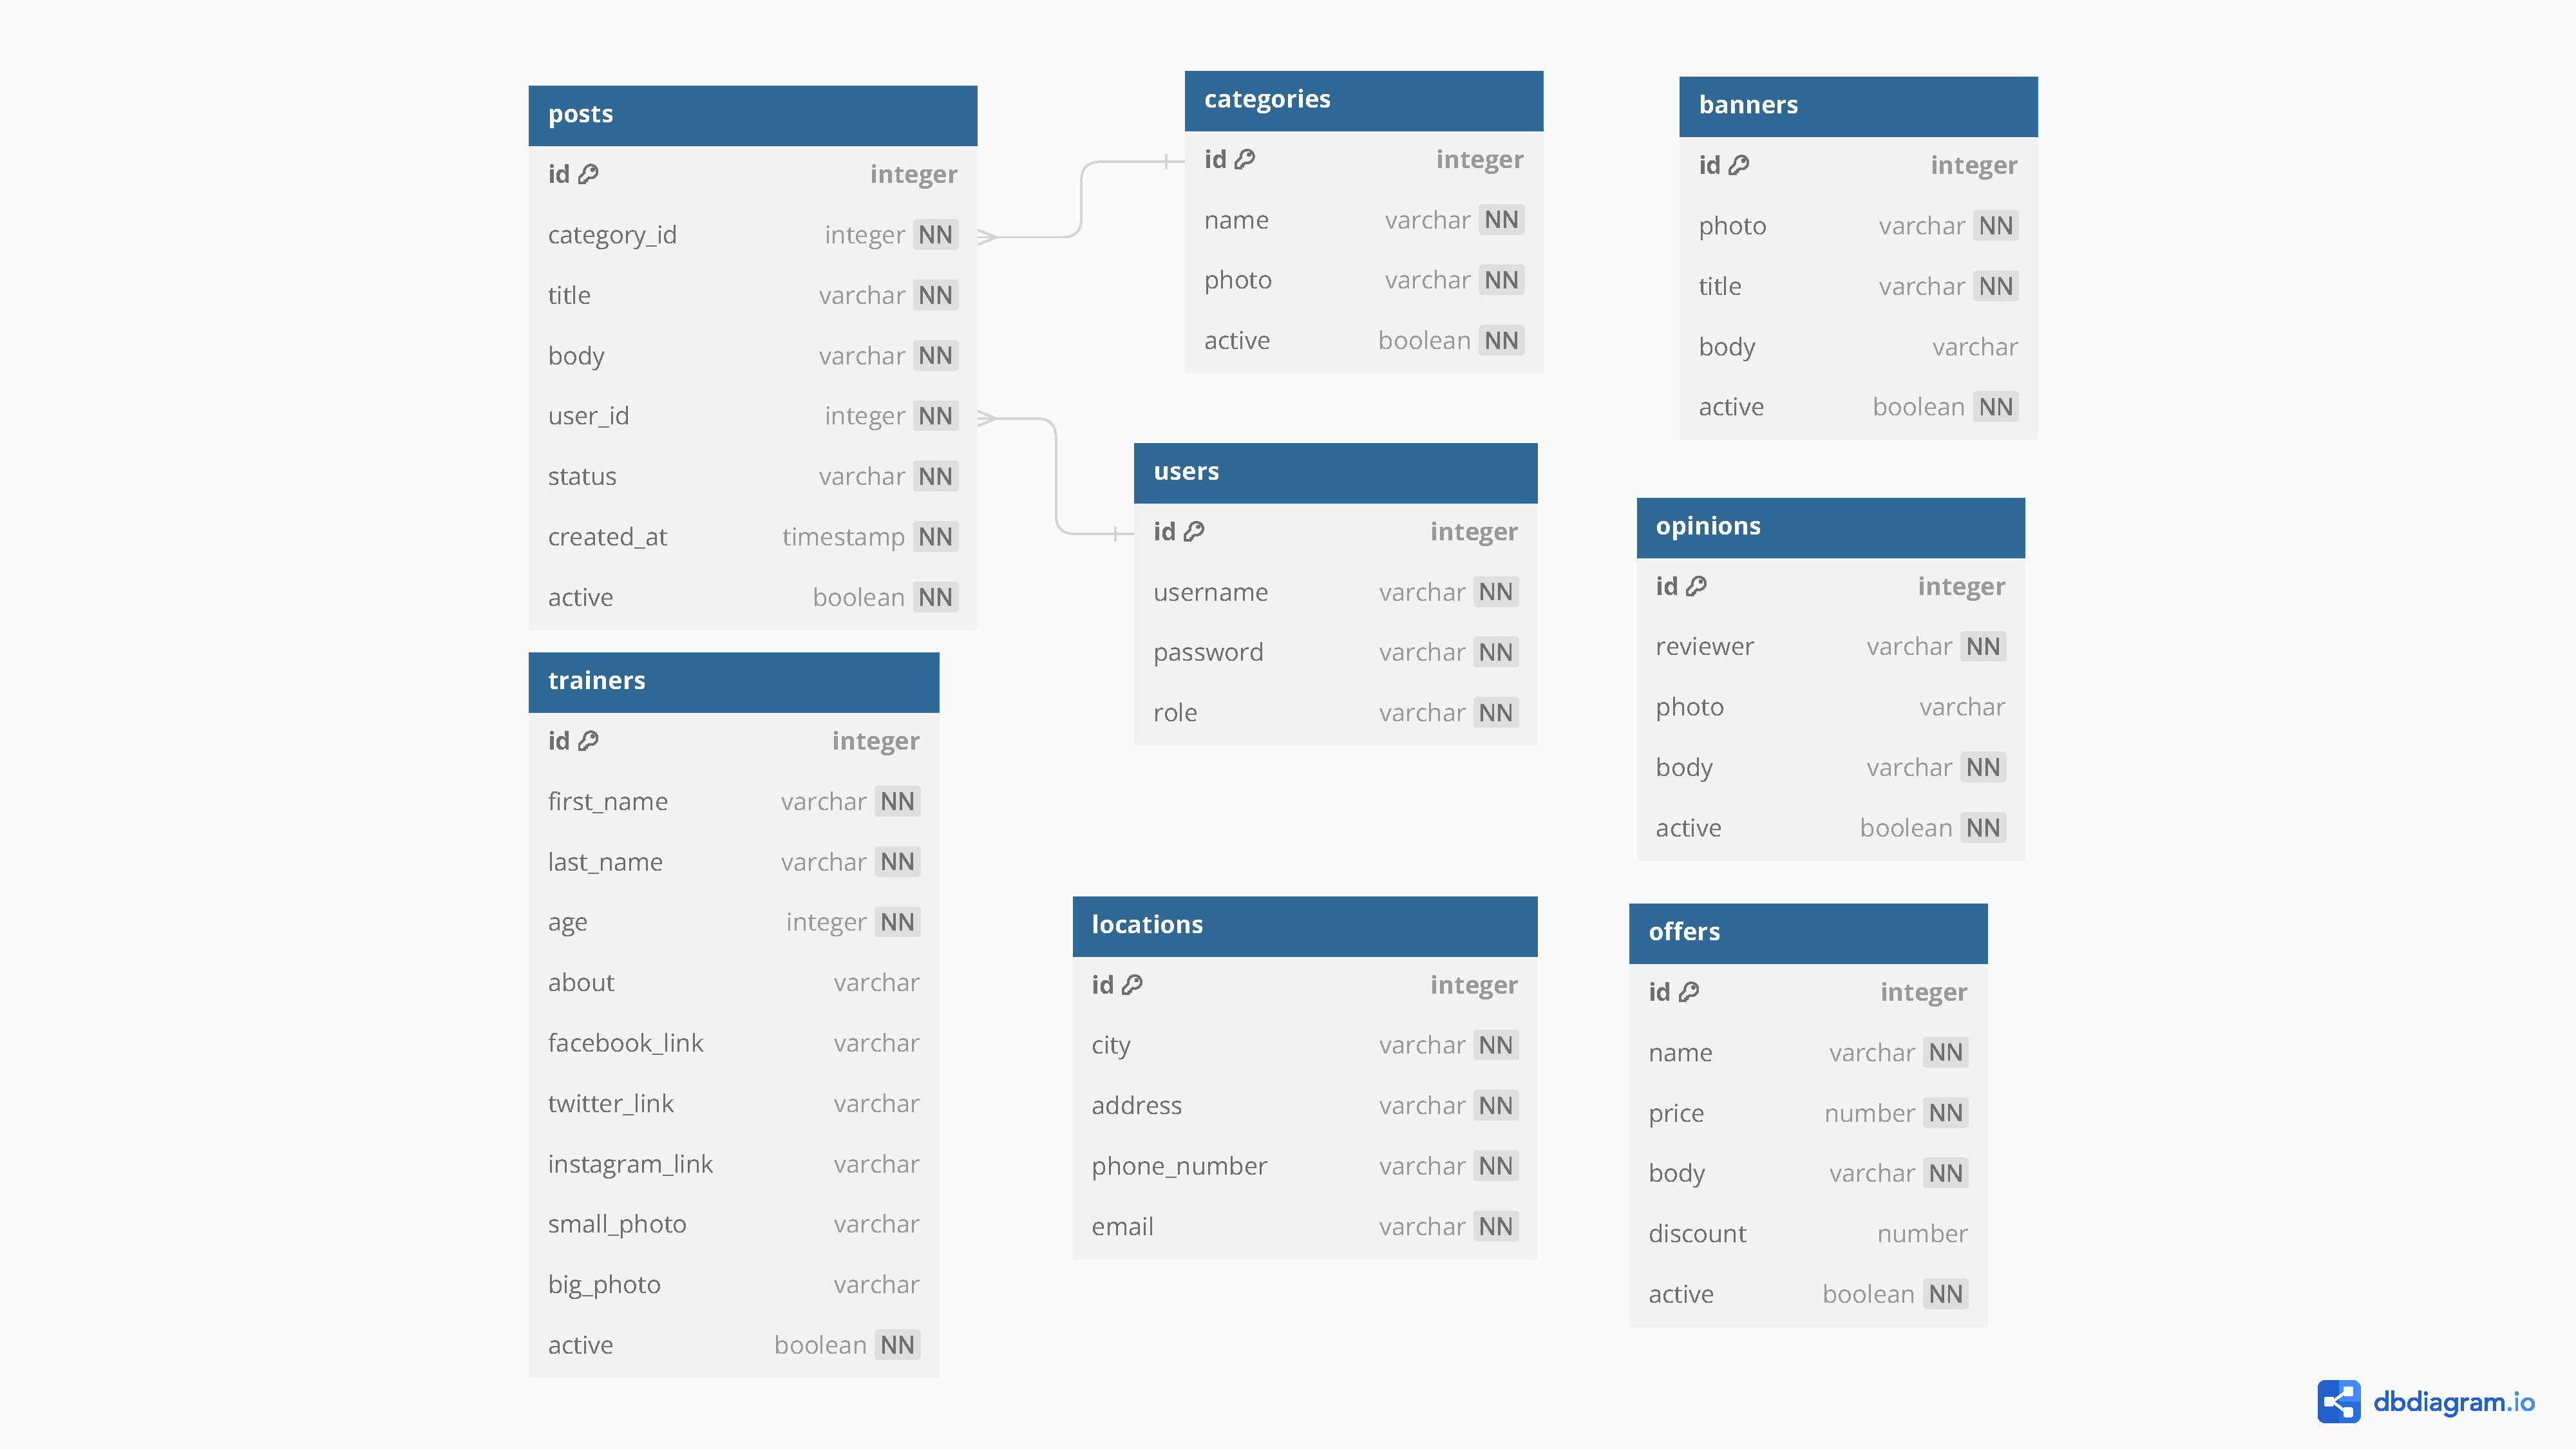
\includegraphics[width=1\textwidth, angle=0]{images/Relational.pdf}
\newpage
\section{Diagram przypadków użycia}
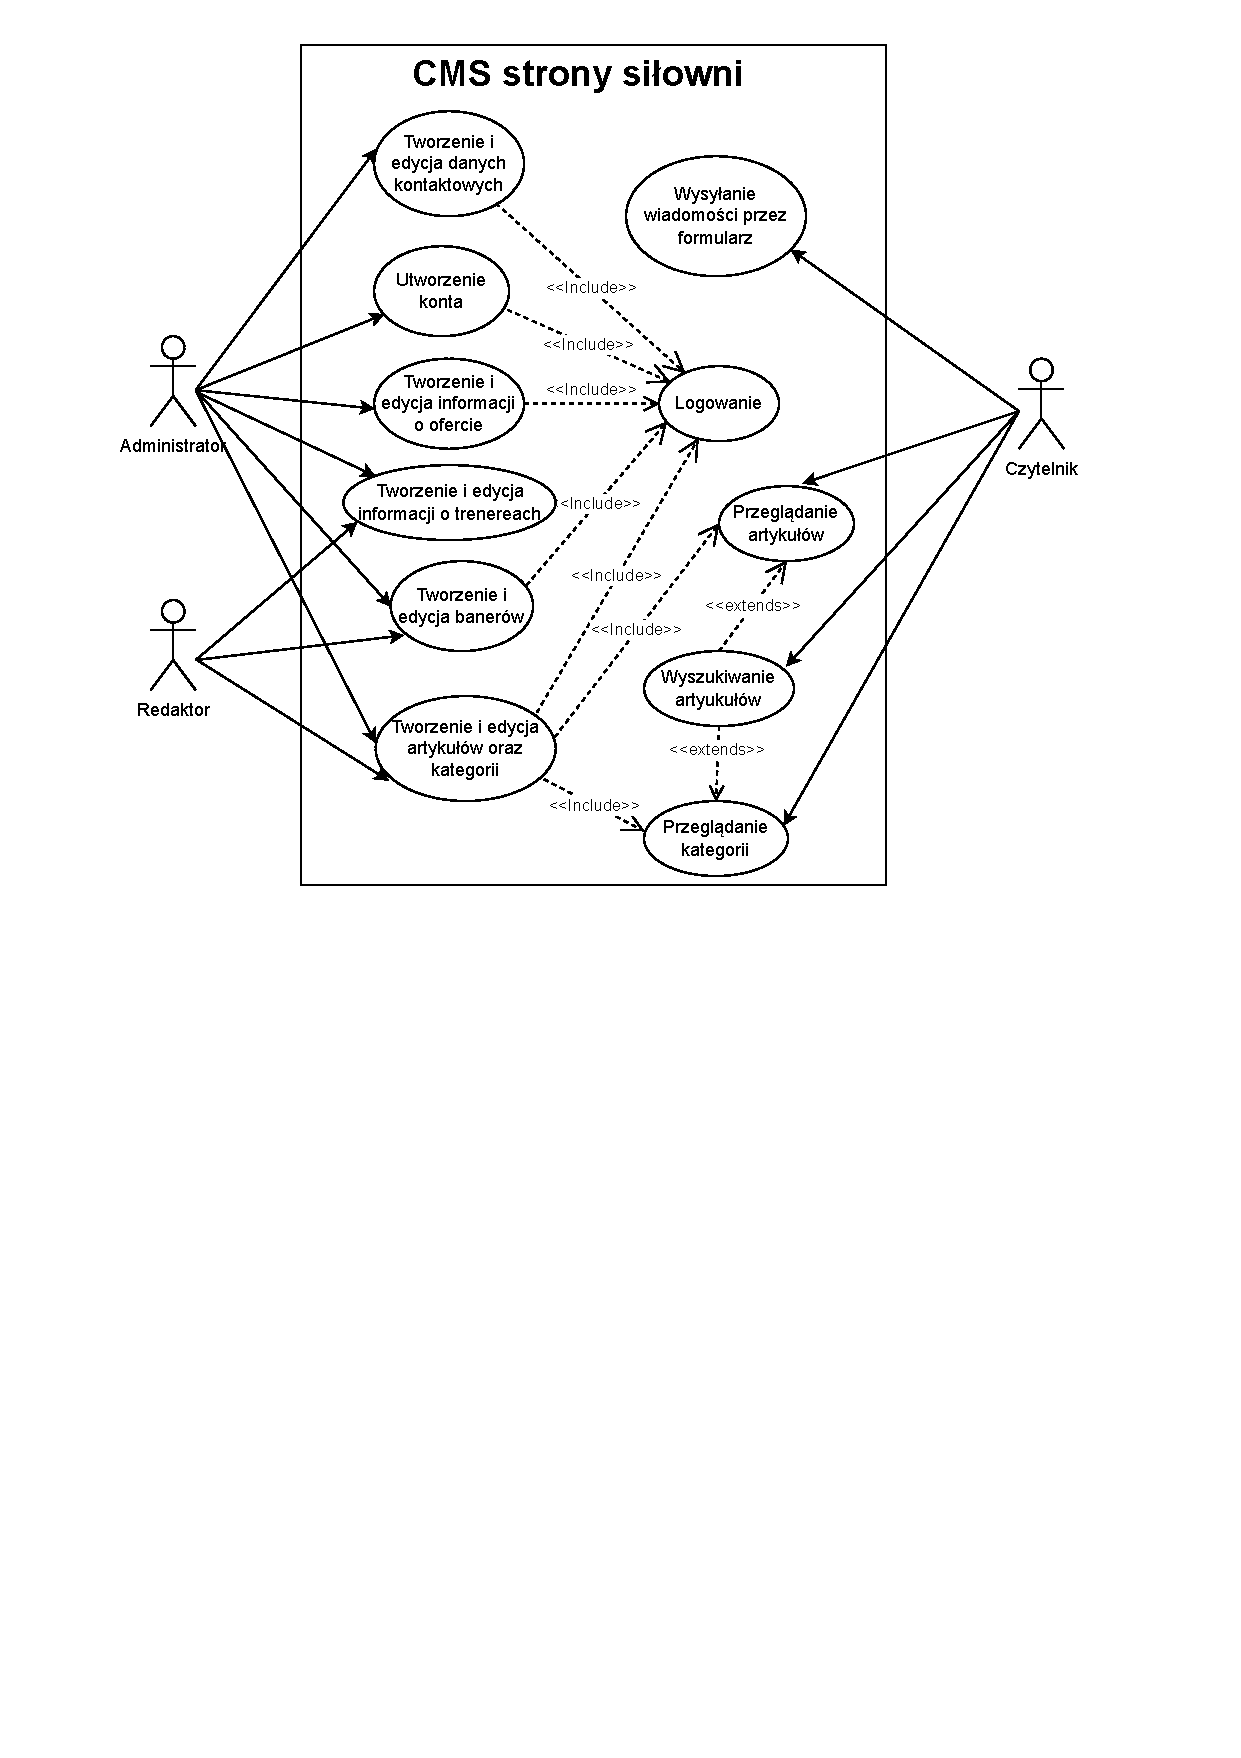
\includegraphics[width=1\textwidth, angle=0]{images/Przypadki_uzycia.pdf}
\newpage
\section{Projekty interfejsu graficznego}
\subsection{Panel administratora}
\subsubsection{Lista elementów}
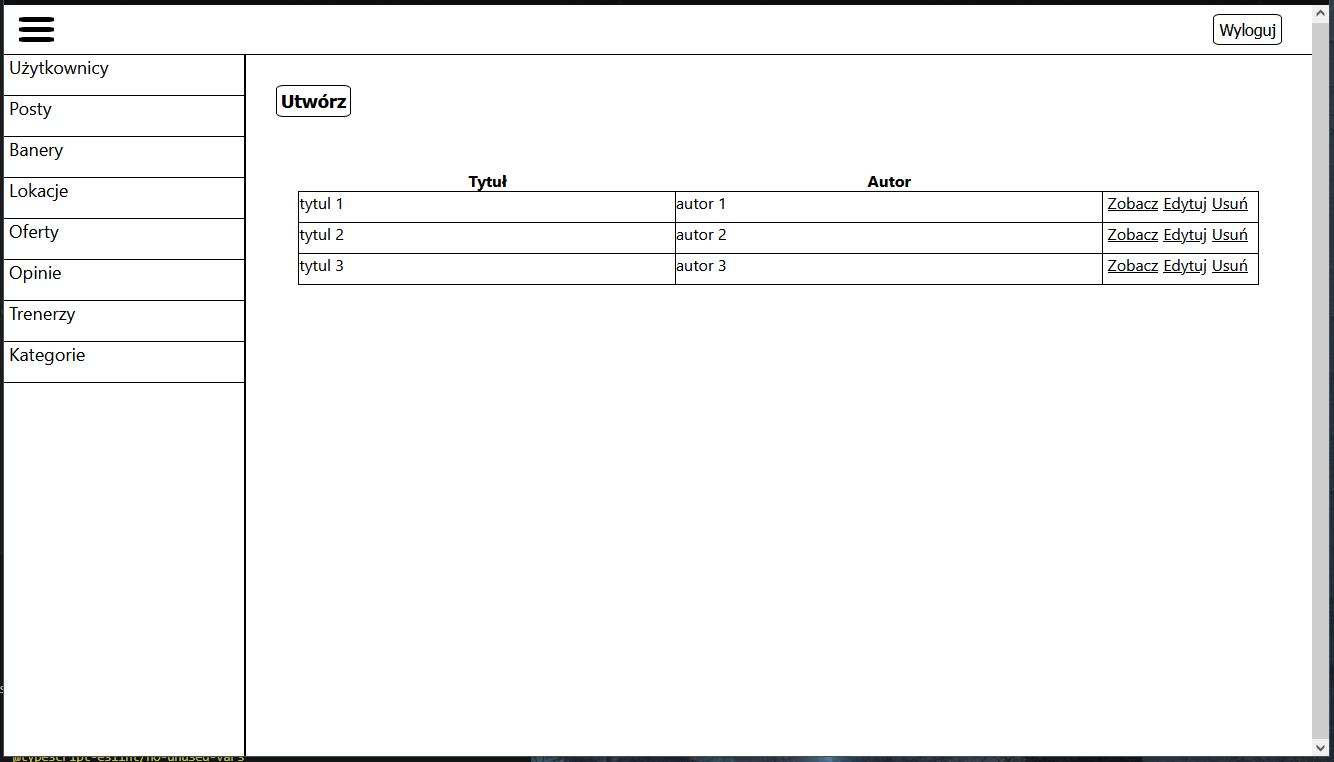
\includegraphics[width=1\textwidth, angle=0]{images/Interfejs_lista.png}
\subsubsection{Ekran logowania}
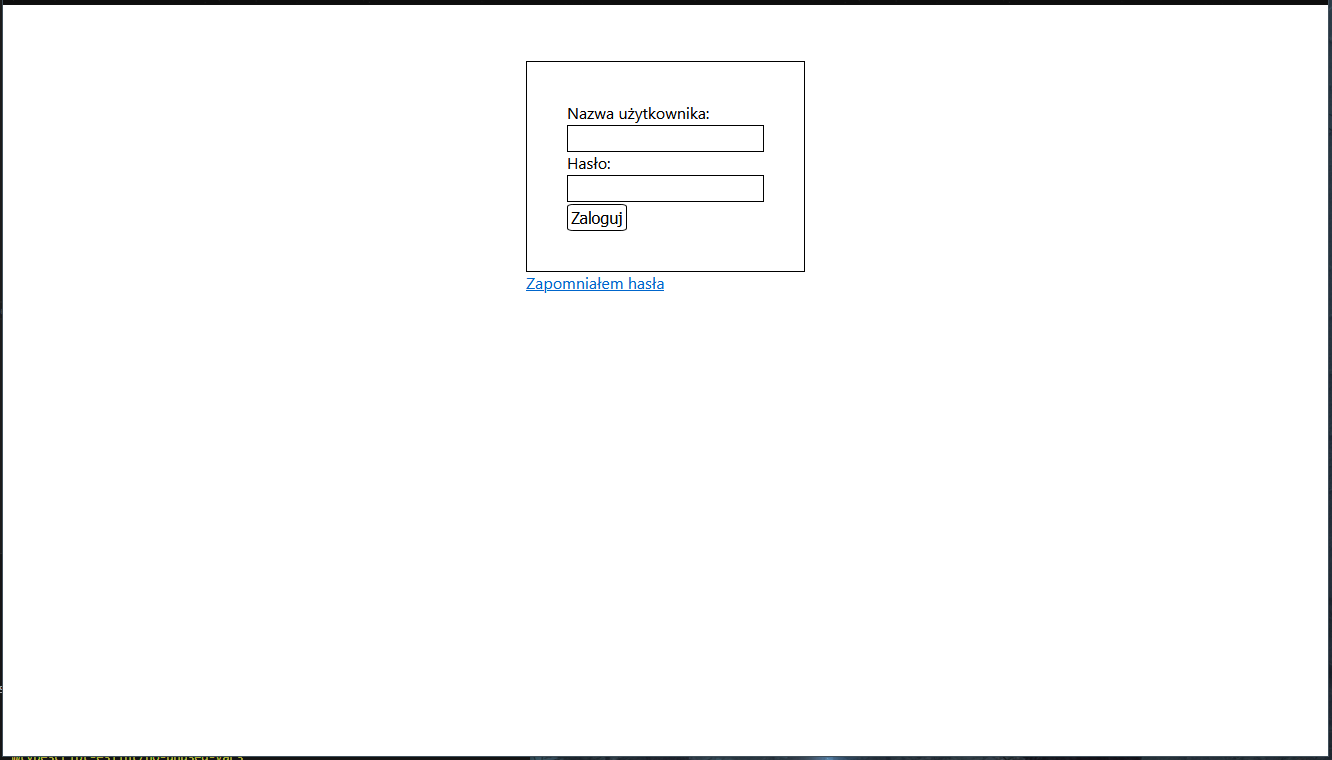
\includegraphics[width=1\textwidth, angle=0]{images/Interfejs_login.png}
\subsubsection{Ekran widoku elementu}
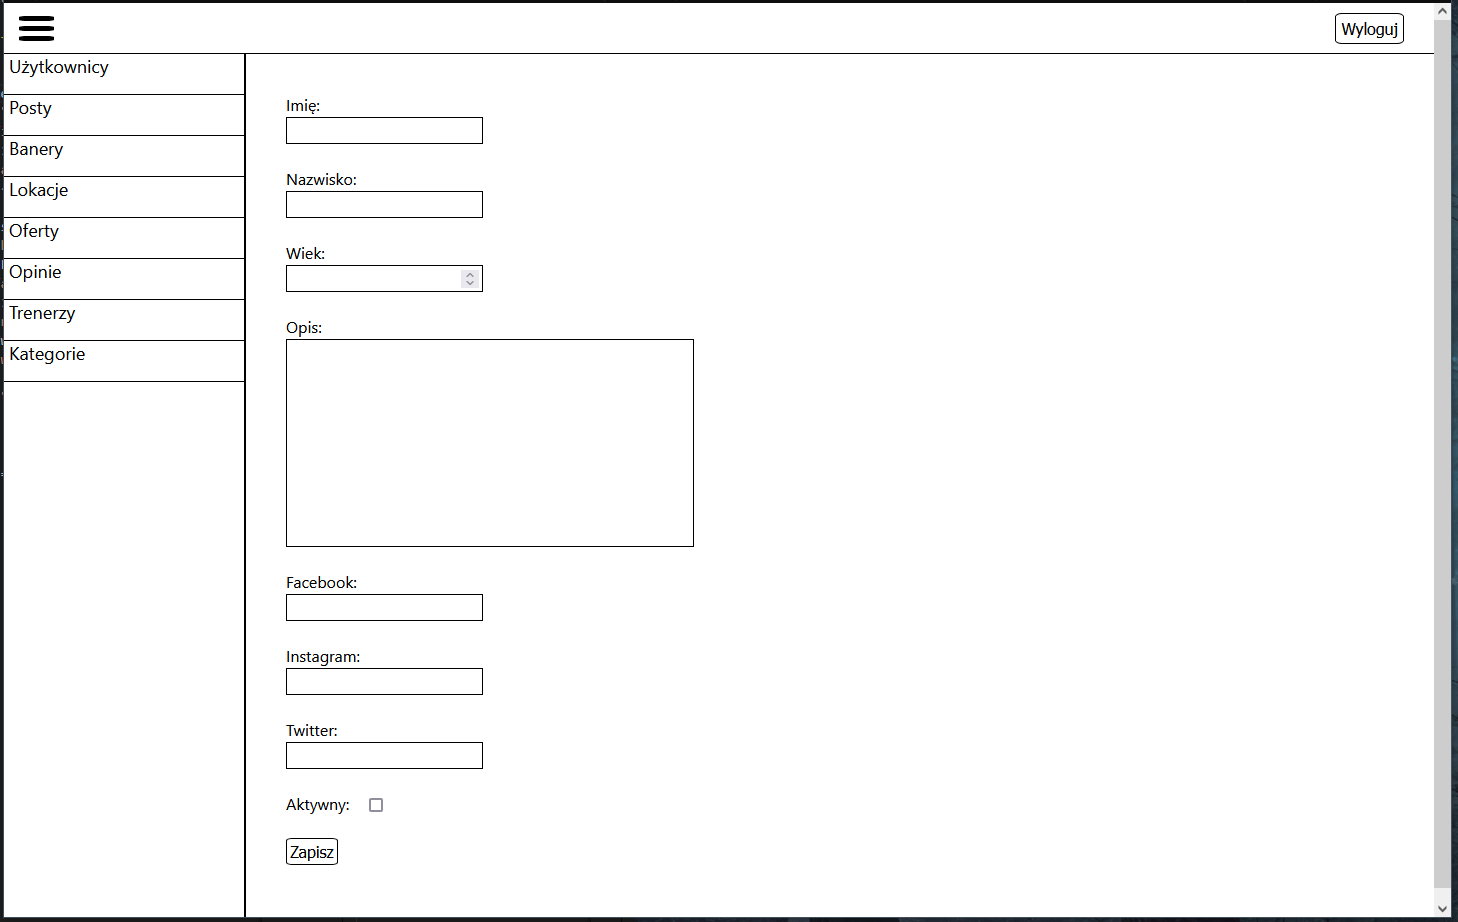
\includegraphics[width=1\textwidth, angle=0]{images/Interfejs_view.png}
\end{document}
